\chapter{Lösungsansatz}
\todoAll{Hier einleitung...}

\section{Idee}
In einer virtuellen Umgebung werden Probanden dazu aufgefordert sich zu entspannen und, nach Möglichkeit, ohne Ablenkung zu verweilen. Das Ziel ist es den Nutzer in einen Zustand der Trägheit zu versetzten, wie er nach dem Schlafen auftreten kann. In diesem Zustand könnten Informationen nur schwer aufgenommen werden und eine Aufgabe, die in diesem Zeitraum gestellt wird könnte so mit geringerem Erfolg erledigt werden, als wenn der Nutzer voll aufnahmefähig ist.

Im Anschluss an die initiale Ruhephase werden die Nutzer auf unterschiedliche Arten `auf\-geweckt' und ihnen wird eine oder mehrere Aufgaben gestellt. Eine Gruppe der Nutzer wird `sanft geweckt' indem die virtuelle Umgebung langsam und bedacht erhellt wird, zudem kann dieser Vorgang mit unterschiedlichen anderen Sinnen unterstützt werden. Die Aufgabenstellung erscheint iterativ und wird mit jedem Schritt anspruchsvoller, bis die volle Schwierigkeit erreicht wurde.
Die andere Gruppe der Nutzer wird hingegen `schnell geweckt'. Hierbei wird die Helligkeit der Virtuellen Umgebung plötzlich erhöht. Auch hier können unterschiedliche Sinne angesprochen werden um möglicherweise den Stressfaktor beim Probanden zu erhöhen. Die Nutzer werden direkt nach dem Aufwachen mit der vollen Schwierigkeit einer Aufgabe konfrontiert und müssen diese lösen.

Im nächsten Schritt des Projekts soll untersucht werden auf welche Arten die Nutzer der beiden Gruppen in dem Erledigen von Aufgaben unterstützt werden können. Hierbei werden vor allem gestalterische sowie aufmerksamkeitssteuernde Aspekte untersucht.

Die Nutzer beider Gruppen können hier dahingehend untersucht werden, mit welchen Fehlerraten sowie welcher Geschwindigkeit die gestellten Aufgaben erledigt werden. Nachfolgend können standardisierte Fragebögen herangezogen werden um das Befinden und die Einschätzung des Nutzers zu untersuchen.

Wir stellen grundlegend die folgenden Hypothesen auf:
\begin{hyp}[H\ref{hyp:schneller}]\label{hyp:schneller}
	Menschen die langsam geweckt werden können sich in kürzerer Zeit auf eine gestellte Aufgabe einstellen, als Menschen, die abrupt aus dem Schlaf gerissen werden.
\end{hyp}

\begin{hyp}[H\ref{hyp:erfolgreicher}]\label{hyp:erfolgreicher}
	Menschen die langsam geweckt werden können eine gestellte Aufgabe mit weniger Fehlern erledigen, als Menschen, die abrupt aus dem Schlaf gerissen werden.
\end{hyp}

und

\begin{hyp}[H\ref{hyp:gestaltung}]\label{hyp:gestaltung}
	Prozedurale Informationen (4C-ID)~\cite{van2002blueprints} bewirken, dass Benutzer eine Aufgabe schneller, sowie mit einer geringeren Fehlerrate erledigen können.
\end{hyp}
\todoAll{Ist diese hypothese noch aktuell? Wir haben ja eigentlich keine prozeduralen Informationen in der Studie untersucht... also raus?}

\subsection{Aufwachen}
Probanden können auf unterschiedliche Arten aufgeweckt werden~\cite{jewett1999time, ferrara2000sleep}
\begin{itemize}
	\item \textbf{Töne}
	\item \textbf{Licht}
\end{itemize}
\todoAll{Beschreiben... und noch auf verwandte Forschung eingehen}

\section{Testaufbau}
Sitzend werden Probanden erst in einen entspannten Zustand versetzt. In diesem verweilen sie möglichst ohne Ablenkung, bis sich eine Gelassenheit oder Trägheit einstellt. Diese kann von entspanntem Sitzen bis hin zum Schlaf führen, eine genaue Zeitspanne hierfür kann zwischen Probanden variieren und muss in Tests bestimmt werden.

Nachfolgend wird der Teilnehmer aus diesem Zustand geleitet und mit einer Aufgabe konfrontiert. Während der Erledigung dieser werden unterschiedliche Parameter aufgezeichnet und später ausgewertet. Die erfassten Parameter sind die folgenden:

\begin{itemize}
	\item Zeit in der eine Aufgabe erledigt wird
	\item Fehlerrate bei der Erledigung der Aufgabe
	\item Blickrichtung
\end{itemize}\todoTob{Redundant mit der Implementierung... wo soll das am ehesten hin?}

Die erste Studie umfasst ungefähr 30 Minuten , hierfür werden die Teilnehmer mit fünf Euro entlohnt. Der Ablauf der Studie Umfasst folgende Punkte:
\todoSab{Hier schreiben, was gemacht wird, nicht was gemacht werden soll. Also Präsens!}
\todoLuc{Hier schreiben, was gemacht wird, nicht was gemacht werden soll. Also Präsens!}

\begin{enumerate}
	\item \textbf{5 Minuten} Vorbereitung und Einführung in den Studienablauf inklusive der Bedienung der VR-Umgebung
	\item \textbf{15 Minuten} Beruhigungsphase bis hin zum Schlafen
	\item \textbf{3-5 Minuten} Aufgaben lösen
	\item \textbf{5 Minuten} Fragebögen beantworten
\end{enumerate}

Die Fragebögen, die wir heranziehen sind zum einen der NASA TLX und ...

Es handelt sich um eine between subject Studie. Im ersten durchlauf erfassen wir die genannten Parameter unter der Betrachtung der Zeit in der die virtuelle Umgebung erhellt wird. Die genauen Zeiten werden in einer Testphase während des Implementierens eingegrenzt.

Zudem werden die Probanden entweder mit Ton oder einer in das VR-Headset eingebauten Temperatureinheit `geweckt'. Auch dieser Parameter wird in einer Testphase experimentell angenähert.

\subsection{Aufgaben}
Die Aufgaben sollen die Aufnahme- und Leistungsfähigkeit der Studienteilnehmer überprüfen. Hierzu wurden Aufgaben gewählt für dessen Erledigung keinerlei Erfahrung mit Virtual-Reality Geräten vorausgesetzt wird. Die Übungen sind verständlich und auch ohne Spielerfahrung bewältigbar. 
% Um die Spiele zu entwickeln können aber auch Toolboxes und Frameworks herangezogen werden, so zum Beispiel auch~\cite{devisch2018mini}.
% Die validierung der Spiele gestaltet sich als schwierig, oder findet jemand noch Quellen? Kann man auch sagen, da es sich nicht um spiele handelt, gestaltet man Aufgaben, die (abstrakt) nahe an eine reale Tätigkeit herankommen? Oder kann man argumentieren, dass hier die gewählten Aufgaben einer realen Tätigkeit entsprechen?
\todoAll{Übergang Idee -> Aufgabe (2-3 Sätze)}

\subsubsection{Zahlenfolge} 
Verteilt über das Blickfeld des Probanden werden Zahlen angezeigt. Die Abstände zwischen den Zahlen sind nicht gleichverteilt und werden idealerweise so gewählt, dass eine Verwechslungsgefahr besteht. Aufsteigend sollen die Zahlen selektiert und so geordnet werden. (123 $\rightarrow$ 324 $\rightarrow$ 823 $\rightarrow$ 1237 ...)

\begin{figure}
	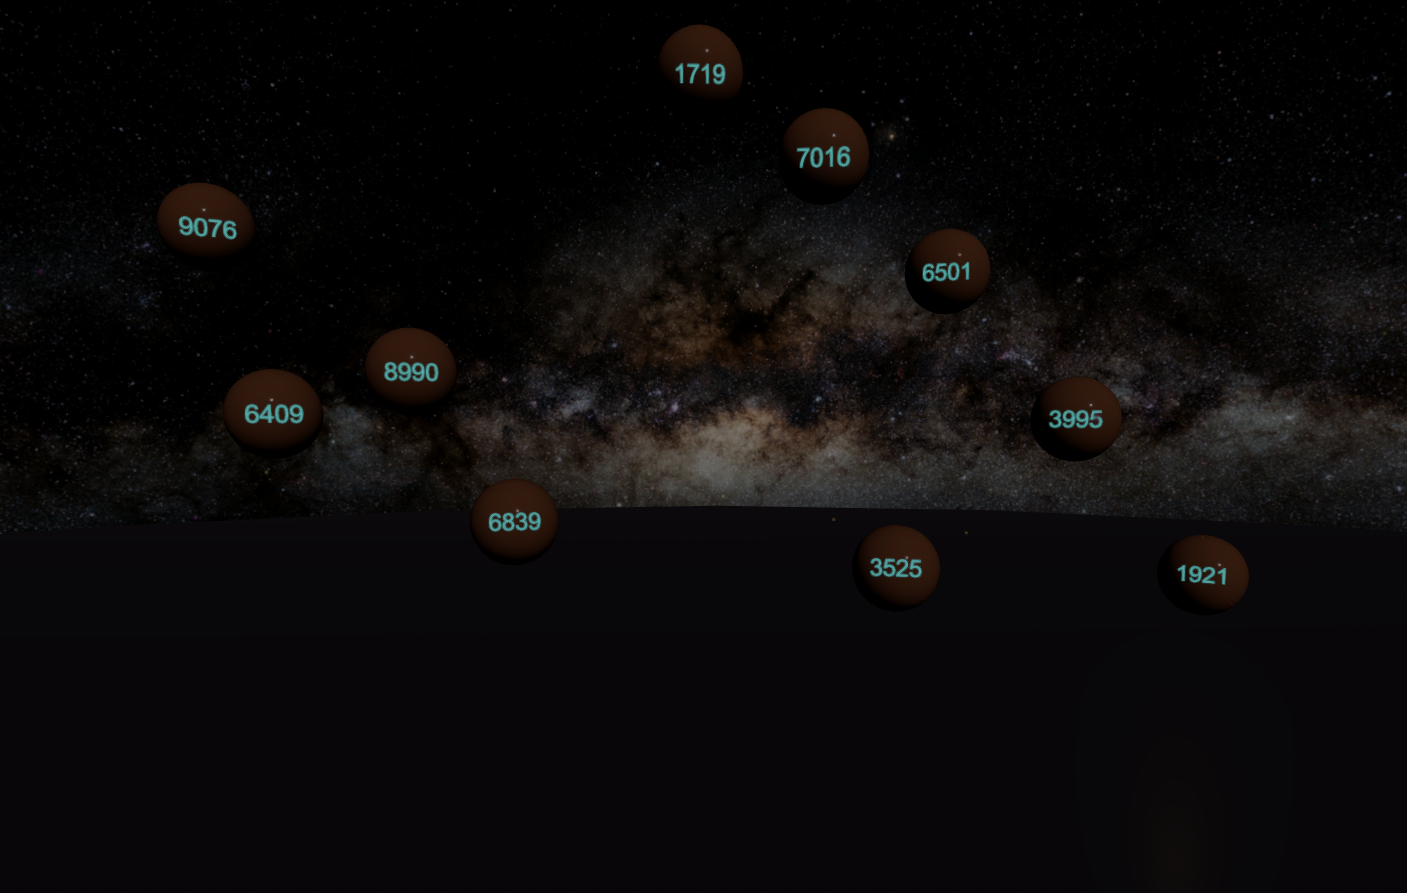
\includegraphics[width=\textwidth]{./images/ordering.png}
	\caption{Erste Aufgabe der Studie. Der Text auf den Kugeln soll in aufsteigender Reihenfolge sortiert ausgewählt werden.}
	\label{fig:ordeing}
\end{figure}

\subsubsection{Stroop-Effekt} 
Im Mittelpunkt des Blickfeldes wird eine ausgeschriebene Farbe angezeigt. Die Textfarbe des Worts muss nicht zwangsläufig die der ausgeschriebenen Farbe sein. Der Proband soll als Eingabe die Textfarbe auswählen indem er mit dem Controller auf einem Interface die richtige Auswahl trifft. Beispiel kann in Figure~\ref{fig:stroop_test} gesehen werden.

\begin{figure}
	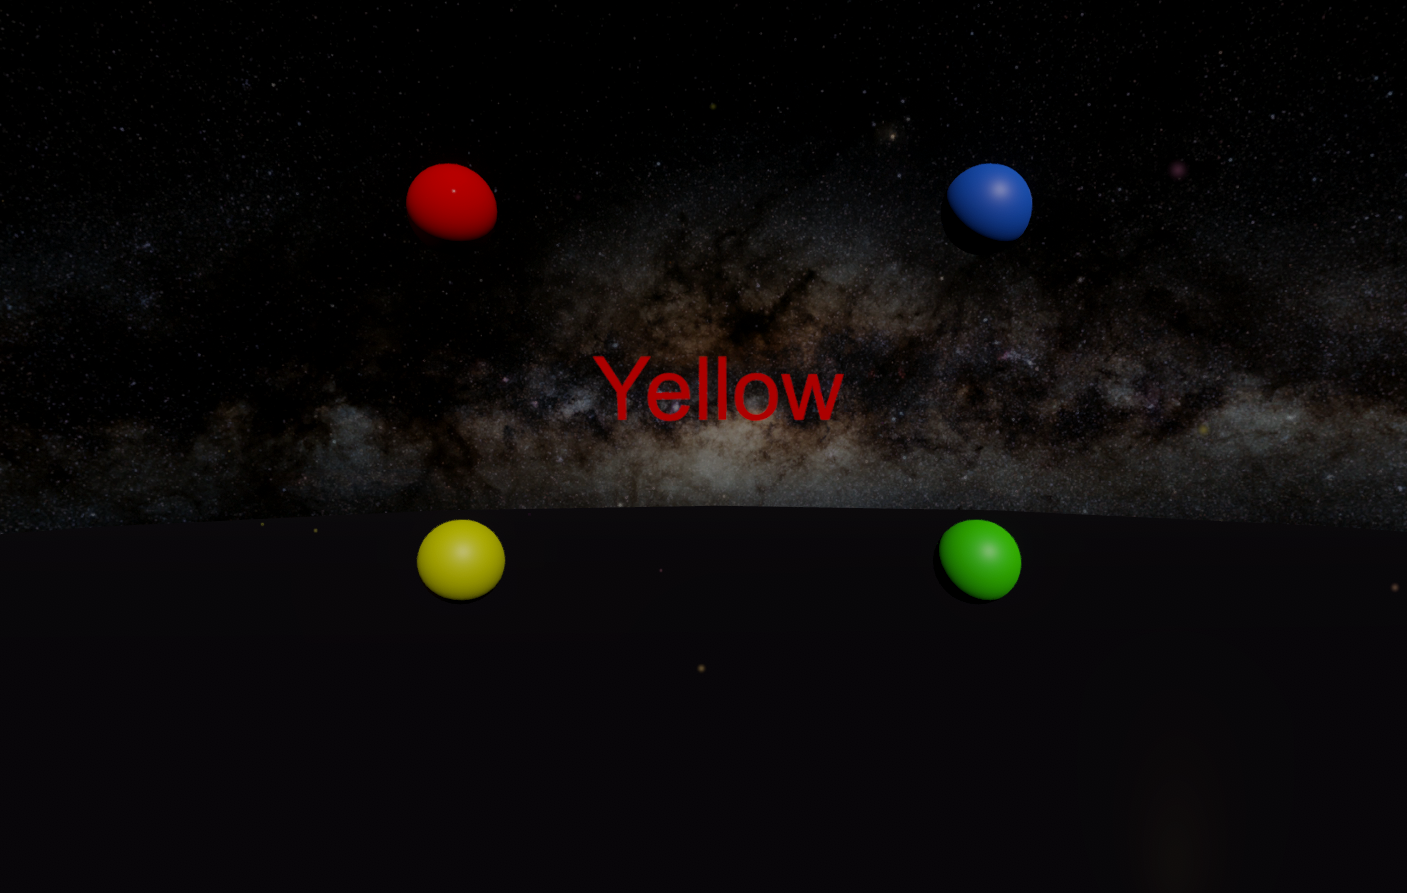
\includegraphics[width=\textwidth]{./images/matching.png}
	\caption{Zweite Aufgabe. Teilnehmer der Studie sollen die Farbe, welche in Textform im Sichtbaren Bereich steht auswählen. Es soll nicht die gleiche Farbe ausgewählt werden.}
	\label{fig:matching}
\end{figure}

\subsubsection{Boxen zählen} 
In isometrischer Ansicht werden eine Vielzahl von Boxen innerhalb der virtuellen Umgebung angezeigt. Die Boxen stehen aufeinander und verdecken zum Teil den Blick auf andere Boxen. Es soll durch die Schlussfolgerung, dass diese, so wie in der realen Welt, nicht in der Luft schweben können, die Anzahl der Boxen gezählt und ausgewählt werden.

\begin{figure}
	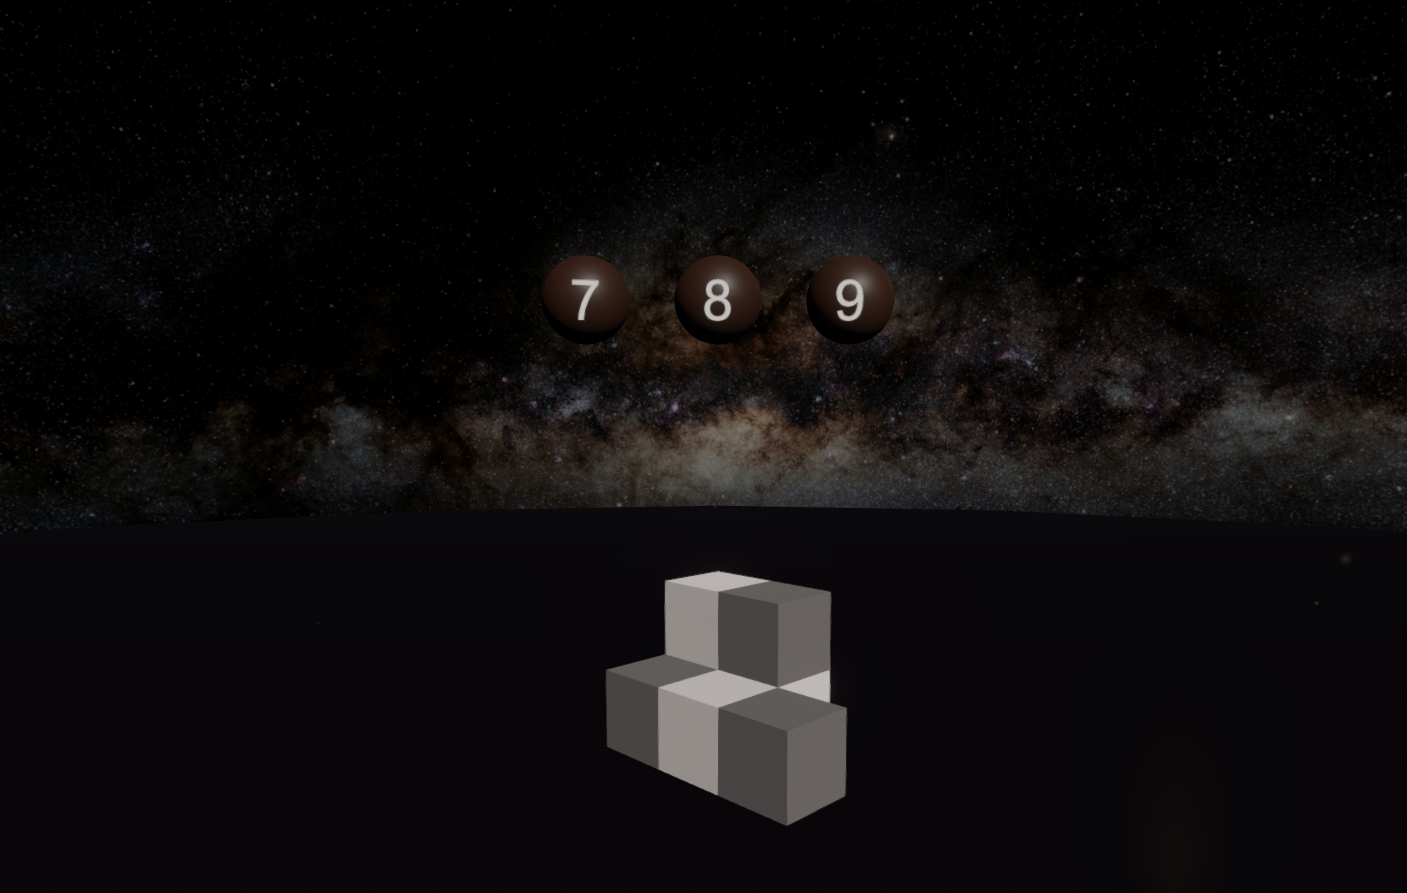
\includegraphics[width=\textwidth]{./images/counting.png}
	\caption{Dritte Aufgabe in der virtuellen Umgebung. Die Teilnehmer sollen die Anzahl der Boxen zählen. Boxen verdecken die sicht auf andere Boxen. Sie können nicht in der Luft schweben.}
	\label{fig:counting}
\end{figure}

%  ===== THIS IS INTENTIONALLY LEFT HERE AS REFERENCE FOR SUBFIGURES (copy&paste)
% \begin{figure}
% 	% \centering
% 	\begin{subfigure}{0.4\textwidth}
% 		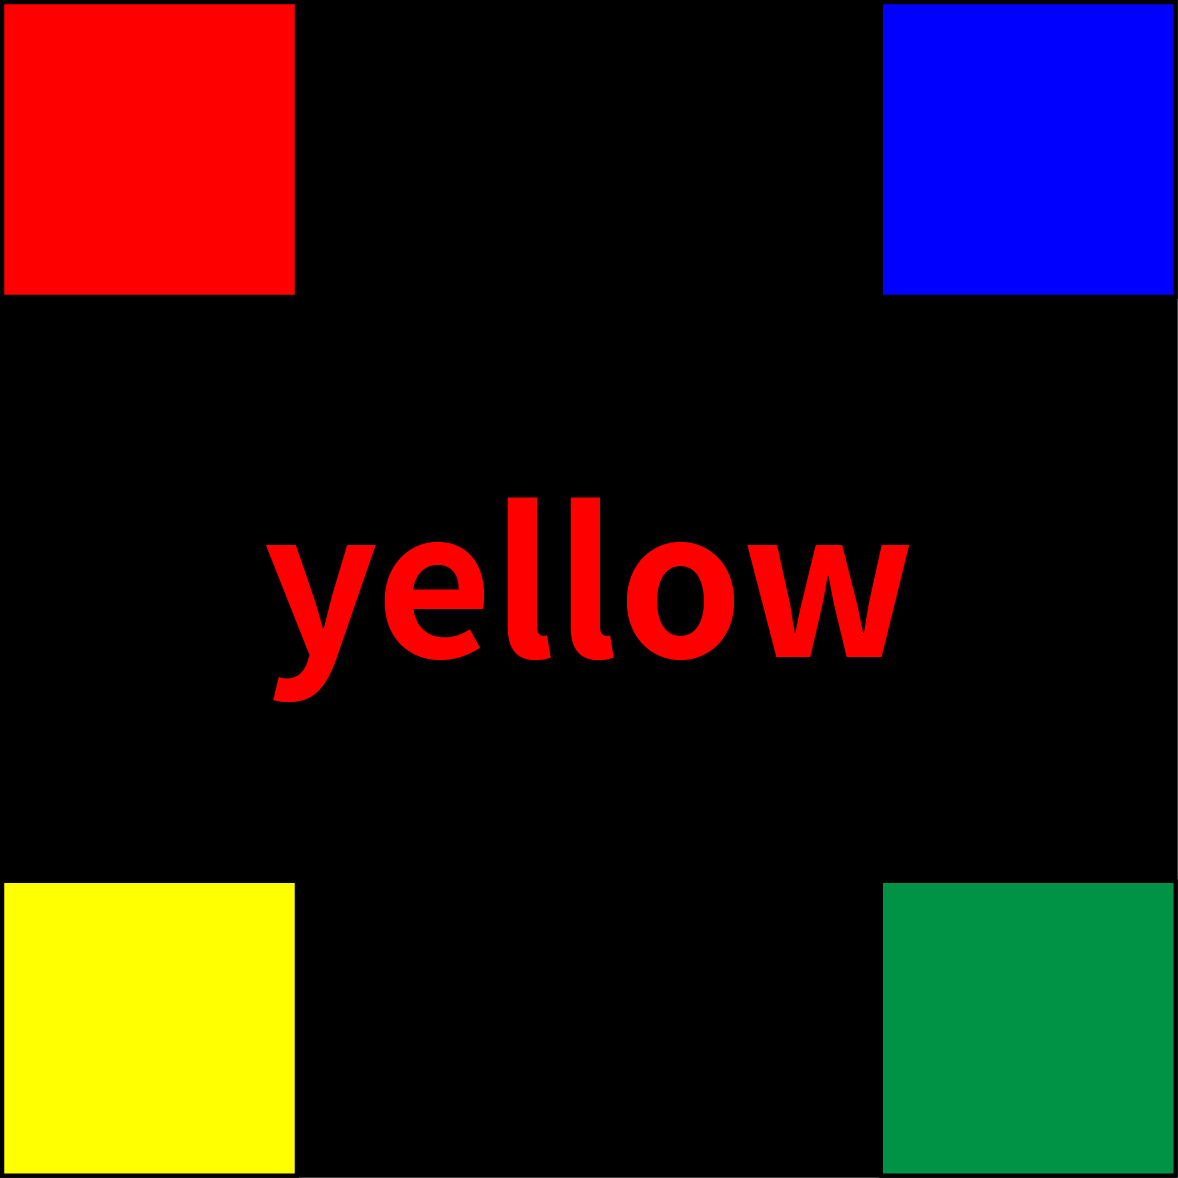
\includegraphics[width=\textwidth]{./images/Reversed_stroop_test.jpg}
% 		\caption{Stroop Test, ElvisLin CC BY-SA 4.0. \url{https://commons.wikimedia.org/wiki/File:Reversed_stroop_test.jpg}} % subcaption
% 		\label{fig:stroop_test}
% 	\end{subfigure}%
% 	\hfill
% 	\begin{subfigure}{0.5\textwidth}
% 		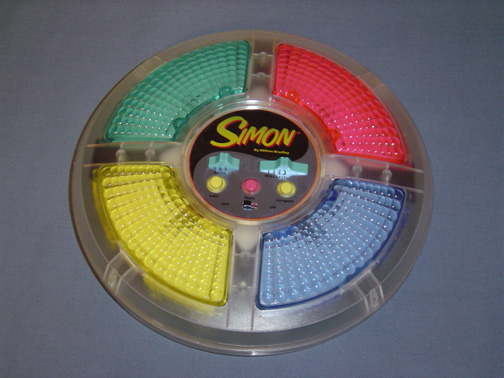
\includegraphics[width=\textwidth]{./images/Simon_game.jpg}
% 		\caption{Senso / Simon, Larry D. Moore CC BY-SA 3.0. \url{https://commons.wikimedia.org/wiki/File:Simon_game.jpg}} % subcaption
% 		\label{fig:simon}
% 	\end{subfigure}
% 	\caption{Beispiele für die Spiele mit denen die Teilnehmer konfrontiert werden.} % caption for whole figure
% \end{figure}
